\documentclass[border=6pt]{standalone}
\usepackage[T1]{fontenc}
\usepackage{lmodern,amsmath,amssymb,bm}
\usepackage{tikz}
\usetikzlibrary{arrows.meta,calc,decorations.pathreplacing}
\begin{document}
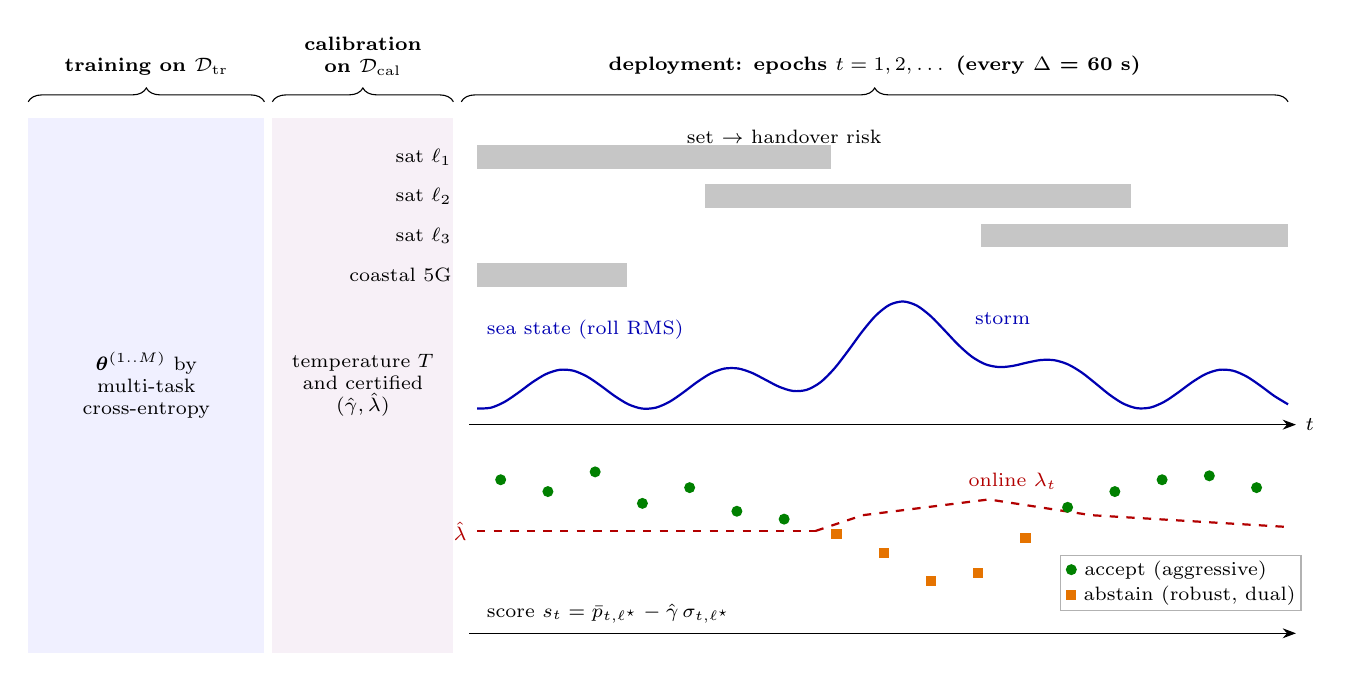
\begin{tikzpicture}[font=\sffamily\small, >=Stealth, x=1cm, y=1cm]
% ---------------- phases
\draw[decorate, decoration={brace, amplitude=5pt}] (0,7.0) -- node[above=6pt, font=\scriptsize\bfseries] {training on $\mathcal D_{\rm tr}$} (3.0,7.0);
\draw[decorate, decoration={brace, amplitude=5pt}] (3.1,7.0) -- node[above=6pt, font=\scriptsize\bfseries, align=center] {calibration\\ on $\mathcal D_{\rm cal}$} (5.4,7.0);
\draw[decorate, decoration={brace, amplitude=5pt}] (5.5,7.0) -- node[above=6pt, font=\scriptsize\bfseries] {deployment: epochs $t=1,2,\dots$ (every $\Delta$ = 60 s)} (16,7.0);
\fill[blue!6] (0,0) rectangle (3.0,6.8); \fill[violet!6] (3.1,0) rectangle (5.4,6.8);
\node[font=\scriptsize, align=center, text width=2.6cm] at (1.5,3.4) {$\bm\theta^{(1..M)}$ by\\ multi-task\\ cross-entropy};
\node[font=\scriptsize, align=center, text width=2.1cm] at (4.25,3.4) {temperature $T$\\ and certified\\ $(\hat\gamma,\hat\lambda)$};
% ---------------- satellite passes
\node[anchor=east, font=\scriptsize] at (5.5,6.3) {sat $\ell_1$};
\node[anchor=east, font=\scriptsize] at (5.5,5.8) {sat $\ell_2$};
\node[anchor=east, font=\scriptsize] at (5.5,5.3) {sat $\ell_3$};
\node[anchor=east, font=\scriptsize] at (5.5,4.8) {coastal 5G};
\fill[gray!45] (5.7,6.15) rectangle (10.2,6.45); \fill[gray!45] (8.6,5.65) rectangle (14.0,5.95);
\fill[gray!45] (12.1,5.15) rectangle (16,5.45); \fill[gray!45] (5.7,4.65) rectangle (7.6,4.95);
\node[font=\scriptsize] at (9.6,6.55) {set $\to$ handover risk};
% ---------------- sea state
\draw[->] (5.6,2.9) -- (16.1,2.9) node[right, font=\scriptsize] {$t$};
\draw[blue!70!black, thick] plot[smooth, domain=5.7:16, samples=60] (\x, {3.35+0.25*sin(deg(3*\x))+ 0.9*exp(-((\x-11.3)^2)/1.5)});
\node[font=\scriptsize, blue!70!black, anchor=west] at (11.9,4.25) {storm};
% ---------------- score vs threshold
\draw[->] (5.6,0.25) -- (16.1,0.25);
\draw[red!70!black, thick, dashed] (5.7,1.55) -- (10.0,1.55) node[pos=0.0, left, font=\scriptsize] {$\hat\lambda$};
\draw[red!70!black, thick, dashed] (10.0,1.55) -- (10.6,1.75) -- (12.2,1.95) -- (13.5,1.75) -- (16,1.6);
\node[font=\scriptsize, red!70!black, anchor=south] at (12.5,1.95) {online $\lambda_t$};
\foreach \x/\y in {6.0/2.2,6.6/2.05,7.2/2.3,7.8/1.9,8.4/2.1,9.0/1.8,9.6/1.7,10.2/1.45,10.8/1.2,11.4/0.85,12.0/0.95,12.6/1.4,13.2/1.85,13.8/2.05,14.4/2.2,15.0/2.25,15.6/2.1}{
  \pgfmathsetmacro{\lam}{(\x<10.0)?1.55:((\x<10.6)?1.55+0.2*(\x-10.0)/0.6:((\x<12.2)?1.75+0.2*(\x-10.6)/1.6:((\x<13.5)?1.95-0.2*(\x-12.2)/1.3:1.75-0.15*(\x-13.5)/2.5)))}
  \ifdim \y pt > \lam pt
    \fill[green!50!black] (\x,\y) circle (0.07);
  \else
    \fill[orange!90!black] (\x,\y) rectangle ++(0.13,0.13);
  \fi
}
\node[font=\scriptsize, anchor=west] at (5.7,0.5) {score $s_t=\bar p_{t,\ell^\star}-\hat\gamma\,\sigma_{t,\ell^\star}$};
\node[font=\scriptsize, align=left, anchor=north west, draw=black!30, fill=white, inner sep=2pt] at (13.1,1.25) {%
\tikz\fill[green!50!black] (0,0) circle (0.07); accept (aggressive)\\[1pt]
\tikz\fill[orange!90!black] (0,0) rectangle (0.13,0.13); abstain (robust, dual)};
\node[font=\scriptsize, blue!70!black, anchor=west] at (5.7,4.1) {sea state (roll RMS)};
\end{tikzpicture}
\end{document}
